\documentclass
[
blockverticalspace=-0.8cm
]
{tikzposter}

\tikzposterlatexaffectionproofoff

\geometry{paperwidth=24in, paperheight=36in}

\makeatletter
\setlength{\TP@visibletextwidth}{23in}
\setlength{\TP@visibletextheight}{35in}
\makeatother

\usepackage[utf8]{inputenc}
\usepackage{tikz}

\usepackage[pangram]{blindtext}
\usepackage{comment}
\usetikzlibrary{arrows.meta}
\newcommand{\largearrow}{-{Latex[length=3mm,width=5mm]}}

\usepackage{setspace}
\onehalfspacing

% Colors sourced from https://www.redcross.org/content/dam/redcross/atg/PDFs/BrandPoster.pdf
\definecolor{coolgray}{HTML}{6D6E70}
\definecolor{redcrossred}{HTML}{ED1B2E}

\tikzset{%
  >={Latex[width=2mm,length=2mm]},
  % Specifications for style of nodes:
            base/.style = {rectangle, rounded corners, draw=black,
                           minimum width=8cm, minimum height=1cm,
                           text centered, font=\sffamily},
		startstyle/.style = {base, fill=blue!30},
		astyle/.style = {base, fill=red!30},
		bstyle/.style = {base, fill=green!30},
		cstyle/.style = {base, minimum width=2.5cm, fill=orange!15,
                           font=\ttfamily},
}

\usecolorstyle[colorOne=coolgray,colorTwo=white,colorThree=redcrossred]{Germany}
\makeatletter
\def\title#1{\gdef\@title{\scalebox{\TP@titletextscale}{%
\begin{minipage}[t]{\linewidth}
\centering
#1
\par
\end{minipage}%
}}}
\makeatother

\onehalfspacing

\title
{
    American Red Cross Analytics for Improvements: \\
    Twitter Fire Emergency Posts
}
%\title{{\Huge American Red Cross Analytics for Improvements: Twitter Fire Emergency Posts}}
%\author{Evan De Broux, David Cho, Rena Haswah, Christopher Millan, Trung Pham, Henry Post, Raul Renteria, Pavan Sistla, Hasani Valdez}
\date{\today}
\institute{Illinois Institute of Technology}
%\begin{block}{Motivation}
%\author{Evan De Broux, David Cho, Rena Haswah, Christopher Millan, Trung Pham, Henry Post, Raul Renteria, Pavan Sistla, Hasani Valdez}
%\end{block}
\usepackage{xcolor}

\begin{document}
\maketitle

\column{1}
\block{Incidents Reported to the ARC \& Response Rate}{}
% \vspace{-1cm}

\begin{columns}

    \column{0.4}
    \block{~}
    {
        \vspace{-5cm}
        \vspace{2cm}

        \begin{center}
            
\includegraphics[scale=1.4]{twitter-graph.png}
        \end{center}
    }

    \column{0.6}
    \block{~}
    {
        \vspace{-5cm}
        
        \begin{tikzfigure}
            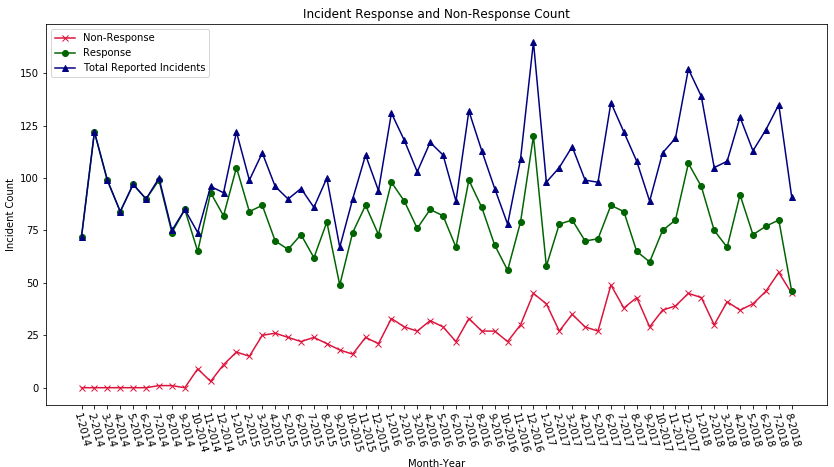
\includegraphics[scale=1.05]{in_response.png}
        \end{tikzfigure}
    }
\end{columns}

\column{1}
\block{Problem Statement}
{
    \fontsize{36pt}{14pt}\selectfont
    The American Red Cross (ARC) responds to an average of nearly 66,000 disasters every year – from a home fire affecting a single household to large emergencies affecting an entire community. Surprisingly, a lot of ARC’s emergency notifications are coming from social media platforms. Currently, they are manually browsing social media posts to find reports of local fire emergencies to respond to. This method is outdated, and can cause some critical posts to be overlooked.

    \begin{tikzfigure}
        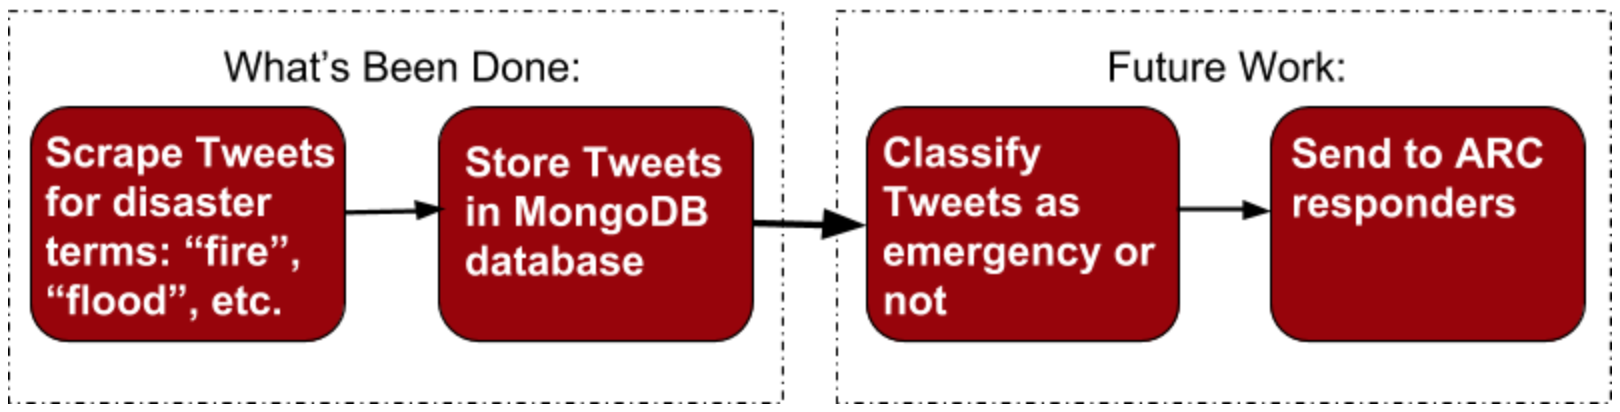
\includegraphics[scale=1.5]{ii.png}
    \end{tikzfigure}

}

\begin{columns}

    \column{0.35}
    \block{Process}
    {
        % First, find all Tweets containing terms that imply disaster, such as ``fire'', ``smoke'', or ``burning''. In order to carry this out, the team developed a Twitter scraping tool that makes use of Twitter’s geotagging feature that allows posters to share their location. Tweets will be used as text files that must be stored in some database to be analyzed for probability of emergency. 
        
        % Once all relevant Tweets are stored in real time, they will be passed through an emergency classifier, that determines whether the post implies a dangerous situation or not. If a post is classified as disastrous, an alert should be sent to all nearby ARC responders.

        \fontsize{36pt}{14pt}\selectfont
        \begin{enumerate}
            \item Find fire-related tweets
            \item Collect and analyze tweets
            \item Detect tweets about an \\\\emergency
            \item Send alerts to responders
        \end{enumerate}
    }
    
    \column{0.65}
    \block{Solution}
    {
        \fontsize{36pt}{14pt}\selectfont
        Ideally, the entire process of searching for local fire emergencies and other disasters would be automated through technology. This optimizes the total amount of Tweets that can be searched through and responded to. Once the occurrence of a disaster is detected, ARC can choose how to allocate volunteers and other resources to best aid the victims. 
    }

\end{columns}

\begin{columns}
% 	\column{0.3}
% 	\block{ARC Responders}
% 	{
%         \begin{tikzfigure}
%             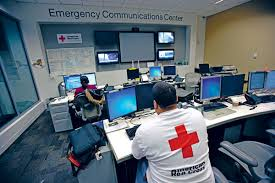
\includegraphics[scale=1.5]{hold.jpeg}
%         \end{tikzfigure}
%     }

	\column{1}
	\block{Product}
	{
        \fontsize{36pt}{14pt}\selectfont
    	The final deliverable would be a service to aid ARC volunteers in finding new local disasters to respond to. The dispatchers would be able to type in a location, and the tool would start to pull all recent disaster-related Tweets within a user specified mileage radius. If something occurs in that region while a volunteer is on duty, an alert would be sent to the volunteers by dispatchers with disaster type and location so that resources could be allocated optimally.  
	}
	
\end{columns}

% Spacing to align authors at end
% \column{1}
% \block{~}
% {
%     \vspace{8cm}
% }


\begin{columns}

	\column{0.55}

    \block{Authors}
        {
            Evan De Broux,
            David Cho,
            Rena Haswah, 
            Christopher Millan,
            Trung Pham, 
            Henry Post, 
            Raul Renteria, 
            Pavan Sistla, 
            Hasani Valdez
        }
    
    \column{0.45}
    \block{}
    {
        \vspace{-1cm}
        
\includegraphics[scale=.5]{Logos.png}
    }
    
\end{columns}



\end{document}
